\documentclass{article}
\usepackage{fullpage}
\usepackage{graphicx}
\usepackage{tabularx}
\usepackage{longtable}
\usepackage{hyperref}

\renewcommand{\arraystretch}{1.5}
\begin{document}
\title{Architecture Documentation Review}
\author{Chiel Peters, Omar Pakker, Mary Gouseti, Cindy Berghuizen}
\maketitle
\setlength\parindent{0pt}
\newcommand{\blank}[1]{\hspace*{#1}}

\section{Introduction}

In this document the architectural solution of the FlyWithUs airline reputation management system is reviewed. The review uses question sets and scenario analysis to determine the completeness
of the architecture. Section two reviews the architecture using premade question sets from \cite{tyree}. In section three multiple scenario's are analysed and how the architecture responds/copes with those scenario's. 

\section{Question sets}

This section contains the answers to the question sets defined in \cite{tyree}. Two question sets where mandatory for this review and the last was specifically taken in order to explain certain limitations in the current version of
the architecture. The first subsection contains questions related to stakeholders and their concerns. In the second subsection the requirements and key design decisions are discussed. Third and final, the viewpoints in the architecture
are reviewed.

\subsection{Question set : Capturing the right stakeholders and concerns}
\begin{longtable}{| l | p{13cm} |}
  \hline
  \textbf{Stakeholder} & \textbf{1. State your stakeholder role. List the set of concerns you have that pertain to the architecture whose AD is being reviewed.} \\
  \hline
  EU Claim & As EU Claim there are two major concerns with the FlyWithUs system. One is that the privacy of the users must be guaranteed. The second is that the system is fair and transparant. No airline should have more influence than another. \\
  \hline
  AirFrance-KLM & AirFrance-KLM wants to be ablo to contact the user based on a review. The customer service wants detailed statistics and reports with regards to both external and internal reviews. Also bad reviews outside of the blame of the Airline companies should not affect the overall rating, hence crossmatching bad weather with flight information should be possible. Other concerns are: costs and customer satisfaction. \\
  \hline
  Dutch Government &As a representative of the Dutch government, Privacy and GreenIT are the main concerns in this project. \\
  \hline
  Initiator & The project must become succesfull in that the FlyWithUs system becomes the  number one airline review website of the web.  My main concerns are the overall functionality of the system, profitability and time to market. \\
  \hline

  \hline
  \textbf{Stakeholder} & \textbf{2. Find and record all places in the AD where your stakeholder role is listed as being covered.} \\
  \hline
  EU Claim & Appendix A, page 16, Stakeholder 2: Sven-Erik Haitjema  \\
  \hline
  AirFrance-KLM & Appendix A, page 16, Stakeholder 4: Sinan Ceylan.  \\
  \hline
  Dutch Government & Appendix A, page 16, Stakeholder 3: Philipp Darkow. \\
  \hline
  Initiator & Appendix A, page 16, Stakeholder 1: Peter Klijn. \\
  \hline

  \hline
  \textbf{Stakeholder} & \textbf{3. Find and record all places in the AD where your concerns are listed as being addressed.} \\
  \hline
  EU Claim & Page 17: R1\\ 
& Page 19: Q4, Q5 \\
  \hline
  AirFrance-KLM & Page 16: F2 \\
    & Page 18: M3 \\
    & Functional Requirements: 5, 8, 9 \\
    & Page 19: Q2\\
  \hline
  Dutch Government & Page 6: GreenIT [R2] \\
    &Page 17: R1\\
    &Page 17: R2 \\
  \hline
  Initiator & Page 6: Vendor lock-in [M2] \\
    & Page 16: F1 \\
    & Page 17: G1 \\
    & Page 17/18: M1 \\
    & Page 18: M2 \\
    & Functional Requirements: 1 t/m 9 \\
    & Page 19: Q1 t/m Q5\\
  \hline

  \hline
  \textbf{Stakeholder} & \textbf{6. Record all concerns you have that are not listed as being covered in either the AD or any framework being used or that are listed in an unclear fashion. For each, state the impact of this omission or misunderstanding on project success.} \\
  \hline
  EU Claim & Both of EU-Claim's concerns are mentioned briefly, but stated in an unclear manner. Transparancy/fairness are mentioned in Q4 however nowhere is mentioned how the system filters the reviews in order to keep the system fair. Privacy is mentioned as logging in and obtaining a certain role. But how privacy works in regards with the all overseeing administrator is not clear. This could become vital for project success if privacy is not well governed (Reputation). \\
  \hline
  AirFrance-KLM & All of AirFrance-KLM concerns are stated except cross-matching the reviews with flight information/weather data. Although not critically important this feature does help the airlines.\\
  \hline
  Dutch Government & Currently the same concern as EU Claim is not covered, how is privacy handled within the system. Are reviews posted with all public information of the user or anonymously? \\
  \hline
  Initiator & As Iniator, the business concerns are clearly covered within the document however the functionality still is unclear. The functional requirements are mentioned however it is not always clear how these will be achieved in the viewpoints. \\
  \hline

  \hline
  \textbf{Stakeholder} & \textbf{7. For each of your concerns as a stakeholder, find and record the places in the AD where that concern is addressed (not just listed). Explain why you do or do not believe that the concern will be satisfied by the architecture.} \\
  \hline
  EU Claim & Privacy: Adressed on page 10 at Airline Rating Service Database on page 25 at seperate users table. The concern related to where the information is placed is clearly stated however how privacy is handled related to reviews is unclear. The user database will be protected and located under dutch law. \\
    & Transparency/Fairness: It is touched upon in page 15 at 'Filter and Store' and at 'Extract and Apply'. However the business rules related to filtering and fairness are not discussed and hence it is hard for the architecture to satisfy this concern. \\
  \hline
  AirFrance-KLM & Usability: Adressed on page 6 at "fast and easy to query"; page 6 at "performance"; page 8 at "B2C application"; page 10 at "Airline Rating Service database"; Section 2.2;  page 18 at "functional requirements"; page 19 at "Quality attribute 2". \newline
  The functional requirements related to AirFrance-KLM are stated in multiple places and this should suffice for the architecture. \\ 
    & Customer contact: Mentioned on page 19 in the requirements however not in the viewpoints. Therefore the architecture will probably not satisfy this concern.  \\
  \hline
  Dutch Government & GreenIT: Adressed on page at "GreenIT [R2]" \newline
  GreenIT is mentioned in the business view. However, it does not give any grounded argumentation or facts for the choice of using a non-relational database. It seems to mostly rely on guesswork and ‘gut-feeling’. The privacy concerns related to the location of the database are clearly stated and the architecture will be able to satisfy this concern. The privacy in the system however is not adressed. \\
  \hline
  Initiator & Functional requirements adressed on page 18. \newline
  The functional requirements are not stated very clear and most of them are not explained in detail through out the viewpoints. The API in the B2C and B2B viewpoints must adress most of these concerns. However the architecture must be defined more in detail to satisfy these concerns. \\
  \hline

  \hline
  \textbf{Stakeholder \blank{.72cm}} & \textbf{8. Find and record the place in the AD that prioritizes the concerns. Explain why you do or do not agree with it.} \\
  \hline
  All & There is no prioritization of the concerns. Some are mentioned in a way that they "must" or "should" be implemented, which may indicate a prioritization. The document in general lays a high focus on how the data is handled which gives a priority to performance and scalability. \\
  \hline

  \hline
  \textbf{Stakeholder \blank{.72cm}} & \textbf{9. Record important stakeholders that you are aware of that are not listed and whose concerns are not represented in the AD.} \\
  \hline
  All & All the stakeholders are listed. \\
  \hline
	
  \hline
  \textbf{Stakeholder \blank{.72cm}} & \textbf{10. State how you know that the architecture satisfies the concerns of the missing stakeholders and where this information can be found in the AD.} \\
  \hline
  All & There are no missing stakeholders. \\
  \hline
\end{longtable}

\newpage
\subsection{Question set : Identify architecturally significant requirements and key design decisions}
\textbf{1. Are specific architecturally significant requirements (i.e., the sub-set of functional, quality attribute, and business requirements that “shape” the architecture under consideration) identified?}

The requirements are stated within Appendix A. They are divided into three subcategories: 
\begin{enumerate}
\item Business Goals
\item Functional requirements
\item Quality attributes
\end{enumerate}

The business goals derive specific requirements related to financial objectives, growth, social responsibility and market position. The business goals are stated using the template in\cite{clemens}. \newline
The functional requirements state the functionality that the system must support. One key requirement of the FlyWithUs system that is not mentioned is the messaging system. Currently the requirements state:

\emph{Business to Business clients need to be able to respond to posts made by Business to Consumer users via the FlyWithUs application}

However this does not capture that the conversation should occur privately between the business and the clients. This would change the architecture as privacy should be considered as a main concern. \newline
The quality attributes state the main quality attributes and how they apply to the system and stakeholders. EU-Claim called for performance however this is not mentioned elsewhere in the document. Privacy and security are taken as one but how privacy applies towards the system is never mentioned.

\vspace{.5cm}
\textbf{2. Are ASRs represented in a clear, unambiguous manner (c.f., 6-part quality attribute scenarios [Bass 2003])? Is the utility of the requirements documented in terms of what the system does and how it meets the customer’s expectations?}

At first, ASRs are introduced and related to the stakeholders. Then they are expressed as business goals, which clarifies these ASRs. However, business goal M3 (\textit{Improve KLM airliner quality in comparison with other}) implies that KLM will be dealt with differently than the other airlines, while one of the requirements states was that all the airlines should be dealt with in the same manner. After the business goals the functional requirements are stated. Functional requirements are expressed as a list of things the system must/should do. However, it is not clear whether or not this vocabulary is used to prioritize the requirements. Additionally the services the system provides to users (business or clients) are briefly mentioned and not elaborated, which makes them unclear. For example, it is mentioned that the data must be fair but it is not explained what that means and how it affects architecture. As a result the system's functionality is not clearly documented which makes it difficult to conclude if it meets the customer's expectations.

\vspace{.5cm}
\textbf {3. Are there remaining requirements that could come up later and have a significant impact on the architecture? How will the architecture (and the architecting process) react to the emergence of new ASRs?}

One big assumption mentioned in the beginning of the document is that the data is not big data. Considering the growth of social networks this may become a requirement in the near future. The current model is a pipeline model which does not easily scale with the amount of incoming data from external sources. Therefore a large part of the ETL module would be required to change in order to cope with the big data.

\vspace{.5cm}
\textbf {4. Is the relationship between ASRs documented and understood (e.g. between performance requirements in a distributed system and the bandwidth reliability and stability of the supporting network transport systems)?}

The relation between scalability and performance is documented and can easily be understood. There are no other relationships mentioned in the requirements.

\vspace{.5cm}
\textbf{5.Are decisions represented in a clear, unambiguous manner (c.f., architectural tactics [Bass 2003])? 
         Is the rationale for key decisions captured?
         Are the costs and resources associated with implementing the decisions documented?}
The main decisions are presented using the template from \cite{tyree}. Apart from the group field that is not correctly used because performance is included in this field, the remaining decisions are clear and unambiguous. The rational of every decision is explained in the argument field. Costs and resources are mentioned but not thoroughly explained.

\vspace{.5cm}
\textbf {6. Are there remaining architectural decisions or impacts (e.g., issues or problems that could come up during deployment, deferred decisions that need to be bound later)?}

Currently for both the B2C and B2B modules all functionality is mentioned as API. There are decisions related to how this API functions what interactions are possible between the modules and the API and how the API obtains the data from the storage. This could be elaborated further to show how functionalities relate and what dependencies there are.

\vspace{.5cm}
\textbf{7. Is there a mapping between decisions and requirements?}
The format used is defined in \cite{tyree}. The table contains the row 'related requirements' which does this mapping. However, it is not followed as strictly as elsewhere in the document where the requirement code (G1, R1 etc.) is used.

\vspace{.5cm}
\textbf{11. Are specific driving architectural decisions identified? Is the relationship between them documented and understood (e.g., between performance requirements in a distributed system and the bandwidth, reliability, and stability of the supporting network transport systems)?}

Most design decisions are based on technical information and less on cost. Therefore they may not be comprehensible to all the stakeholders. The format used is defined in \cite{tyree} and contains a row 'related design decisions' which indicates with decisions are related. How they are related is however not mentioned.

\vspace{.5cm}
\textbf{12. Are decisions represented in a clear, unambiguous manner? Is the rationale for key decisions captured? Are the costs and resources associated with implementing the decisions documented?}
Arguments and implications are provided for most of the main decisions, which makes their significance clear to the stakeholders. However, the costs are not analysed enough.

\vspace{.5cm}
\textbf{13. Are there remaining architectural decisions or impacts (e.g., issues or problems that could come up during deployment, deferred decisions that need to be bound later)?}

As mentioned towards the architects there are remaining design decisions related towards the functionality of the B2B and B2C modules and how these modules are communicating.

\vspace{.5cm}
\textbf{14. Do you understand how the AD will identify constraints and implementation responsibilities (e.g. delegated decisions?)}

The constraints are given in the template of \cite{clemens} in the row 'constraints'. However, the implementation responsibilities are not identified.
%However, the responsibilities are not delegated towards the stakeholders. This is because only the stakeholders that use the system are mentioned and not the stakeholders that will implement this system.


\newpage
\subsection{Question set : Reviewing the choice of Viewpoints}
This subset of questions is based of \emph{Reviewing Choice of Framework and Viewpoints} (\cite{tyree}). Only the questions related to viewpoints and views are chosen, because the AD is not developed within any specific framework.\\

\textbf{1. Do the selected viewpoints and their prescribed models, languages, techniques, evaluation criteria, correspondence rules, and so on, frame the concerns of the stakeholders?}

The selected viewpoints in this case are the Business view, the functional decomposition view and a view of the datastore. This should frame the concerns of the stakeholders. The business view frames the concerns of the initiator, the Dutch government and Airfrance-KLM, the functional view frames the concerns of Airfrance-KLM and the initiator and the ETL Pipes-and-Filter view also frames the concerns of the Initiator. There is no view that will represent the concerns of EU claim and the concerns about privacy are missing in the viewpoints. 
 
\vspace{.5cm}

\textbf{9. For each viewpoint, are its models clear and well-defined? Do the models provide enough information for determining whether the concerns framed by the viewpoint have been satisfied?}

The viewpoints all use seperate symbols and do not all contain a legend which make some models unclear. The models could benefit from a consistent symbol use through out the (sub) viewpoints.

The first view is the business goal view which frames the concerns of the initiator, the Dutch Government and Airfrance-KLM. The business view gives a readable overview of the options when choosing a database system, which is important for the performance, time to market and the profit to be made. The view also shows GreenIT, which is a concern of the Dutch Government. \\

The second view presented is the functional decomposition view.  This view should satisfy the concerns of AirFrance-KLM and the initiator. Although it gives a nice overview of the system and considers the modifiability of the program, the view is too general. The functionalities of the system like the reporting / reviewing and messaging system are nowhere to be found. The document zooms in on different aspects of the functional viewpoint, but it still does not frame all the concerns. The datastore zoom gives a good view for how the data is handled but for framing all the stakeholders concerns the B2B/B2C zoom should be more specific. The conclusion is that although this view is important to be presented, it is not detailed enough to give a good representation of the functionalities of the system.\\

The third view is the ETL Pipes-and-Filter view and focuses on Q1 (modifiability) and Q4 (data quality) which are mainly concerns of the initiator. In this view it becomes clear how the Data-Source adapters contribute to the modifiability of the system, which is very important for FlyWithUs. Also, it gives a clear view of how the incoming data is handled and stored. 
\vspace{.5cm}

\textbf{11. What correspondences exist between models in the same viewpoint or across different viewpoints? Which came from the architect's own selection of viewpoints?}

The functional decomposition view and the ETL Pipes-and-Filter have a lot of simularities. As indicated on page 7 the ETL Pipes-and-Filter view was originally intended to be inside the functional decomposition view as a seperate subsection (2.3). The architectures however found that the ETL was better placed in its own view. 

\vspace{.5cm}

\textbf{14. Is it feasible that the views drawing upon these models, viewpoints, and framework(s) can be constructed with the available tool, techniques, and people within the time and funding available?}

Because of the high level of technicality within the current viewpoints it is likely that the views can be constructed with the available tools and techniques. The time frame is stated as 6 months (requirement M1 on page 17), how this goal is achieved is however not mentioned within the views and needs be further researched. 
\vspace{.5cm}

\textbf{15. Is there rationale captured for the choice of framework, viewpoints, models, and correspondences?}

The rationale for the choice of viewpoints is not stated in the architectural documentation.
\newpage
\section{Scenarios}

This section contains four scenario's and how the architecture responds to them. The format is obtained from \cite{clemens}. The choices for scenario's were made on multiple factors:
\begin{enumerate}
\itemsep0em 
\item To demonstrate one of the key design decisions and the related trade-offs and sensitivity points (\ref{sec:failureb2b})
\item To indicate that some (implicit) design decisions are still open for discussion (\ref{sec:peakload},\ref{sec:privacy})
\item To test how the architecture responds to a change in an assumption and which components need to be modified (\ref{sec:bigdata})
\end{enumerate}

\subsection{Scenario: Failure in B2B/B2C} \label{sec:failureb2b}
\begin{tabularx}{\textwidth}{| l | X |}
  \hline
  \textbf{Scenario} & B2B - B2C decoupling \\
  \hline
  \textbf{Attribute} & Availability \\
  \hline
  \textbf{Environment} & Normal Operations \\
  \hline
  \textbf{Stimulus} & B2B or B2C failure \\
  \hline
  \textbf{Response} & Failure of either one does not influence the other. \\
  \hline
    &
    \begin{tabular}[t]{ | @{}| p{4cm} | l | l | l | l | @{} | }
      \hline
      \textbf{Architectural Decision} & \textbf{Sensitivity} & \textbf{Tradeoff} & \textbf{Risk} & \textbf{Non-risk} \\
      \hline
      Decoupling & S1 & T1 & & \\
      \hline
      Different API & S1 & T2 & & N1 \\
      \hline
    \end{tabular}
    \\
    &  T1: When both systems are decoupled and both access the same data store a tradoff is created. The performance of the B2C clients is directly linked to the performance of the B2B clients \newline
    T2: The API contains duplicate functionality hence redundant code might exist. This is a trade off between modifiability/maintainability because of the redundant code vs availability (one system crashes does not influence the other system). \newline
    N1: If the API was not split up as well then this would create a single point of failure as mentioned by the architecs. \newline
    S1: If the B2B and B2C systems  are in the same server and the server goes down, B2C and B2B will both go down. \\
  \hline
  \textbf{Reasoning} & Decoupling ensures, together with the different API, that if one the B2B or B2C module goes down, the other won't. \\
  \hline
  \textbf{Architecture Diagram} & The red API crashes. \\
   & 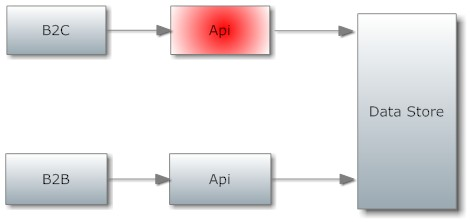
\includegraphics[width=250px]{scenario1} \\
  \hline
\end{tabularx}

\subsection{Scenario: Peak load on analytics module} \label{sec:peakload}

\begin{tabularx}{\textwidth}{| l | X |}
  \hline
  \textbf{Scenario} & Peak load on the analytics module \\
  \hline
  \textbf{Attribute} & Performance \\
  \hline
  \textbf{Environment} & Normal Operations \\
  \hline
  \textbf{Stimulus} & Recalculating ratings/reviews \\
  \hline
  \textbf{Response} & B2B latency <10 sec. \\
  \hline
    &
    \begin{tabular}[t]{ | @{}| p{4cm} | l | l | l | l | @{} | }
      \hline
      \textbf{Architectural Decision} & \textbf{Sensitivity} & \textbf{Tradeoff} & \textbf{Risk} & \textbf{Non-risk} \\
      \hline
      Recalculate 1/2 times a day (Implicit) & & & R1 & \\
      \hline
      B2B accesses analytics directly (Implicit) & & T1 & & \\
      \hline
    \end{tabular}
    \\
    & R1: Recalculating the final rating once or twice a day creates a major peak load on the analytics module and might lead to an unavailable analytics module for the B2B clients. \newline
    T1: B2B clients can directly access the analytics module, this gives the B2B clients the freedom to perform custom searches, but also leads to unavailability if the module is overburdend.\\
  \hline
  \textbf{Reasoning} & Recalculating on a time frame creates a massive peakload  which may lead to an undesirable response time when the B2B performs a custom search. \\
  \hline
  \textbf{Architecture Diagram} & Analytics module overloaded. \\
   & 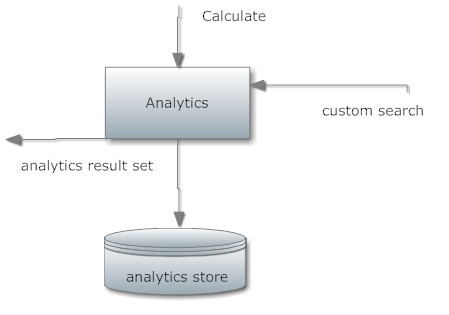
\includegraphics[width=300px]{scenario2} \\
  \hline
\end{tabularx}

\subsection{Scenario: Review privacy} \label{sec:privacy}

\begin{tabularx}{\textwidth}{| l | X |}
  \hline
  \textbf{Scenario} & Review Privacy \\
  \hline
  \textbf{Attribute} & Privacy \\
  \hline
  \textbf{Environment} & Normal Operations \\
  \hline
  \textbf{Stimulus} & User writes a review \\
  \hline
  \textbf{Response} & Anonymous review \\
  \hline
    &
    \begin{tabular}[t]{ | @{}| p{4cm} | l | l | l | l | @{} | }
      \hline
      \textbf{Architectural Decision} & \textbf{Sensitivity} & \textbf{Tradeoff} & \textbf{Risk} & \textbf{Non-risk} \\
      \hline
      Logged In & & & R1 & \\
      \hline
    \end{tabular}
    \\
    & R1: The anonymity of the user posting a review is not guaranteed.  \\
  \hline
  \textbf{Reasoning} & In the architecture it is not stated that a review will be shown anonymous or how anonimity of reviews is guaranteed. \\
  \hline
  \textbf{Architecture Diagram} & Anyone can see review details. \\
   & 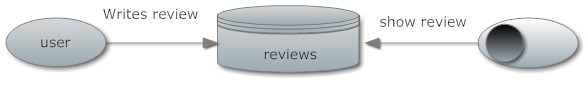
\includegraphics[width=300px]{scenario3} \\
  \hline
\end{tabularx}

\subsection{Scenario: Big data} \label{sec:bigdata}

\begin{tabularx}{\textwidth}{| l | X |}
  \hline
  \textbf{Scenario} & Big Data \\
  \hline
  \textbf{Attribute} & Performance, Availability \\
  \hline
  \textbf{Environment} & Normal Operations \\
  \hline
  \textbf{Stimulus} & Big Data input \\
  \hline
  \textbf{Response} & Handle all input without any loss of data. \\
  \hline
    &
    \begin{tabular}[t]{ | @{}| p{4cm} | l | l | l | l | @{} | }
      \hline
      \textbf{Architectural Decision} & \textbf{Sensitivity} & \textbf{Tradeoff} & \textbf{Risk} & \textbf{Non-risk} \\
      \hline
      ETL Adapters & & & & N1 \\
      \hline
      ETL Approaches & S1 & & & \\
      \hline
      Pipeline Structure & & & R1 & \\
      \hline
    \end{tabular}
    \\
    & S1: If it is Big data the system can not handle the input a choke point will occur in the pipe model. \newline
    N1: The modules in the ETL are independent and therefore easily modifiable. \newline
    R1: The \emph{Filter and Store} and \emph{Extract and apply} module process all reviews sequentially which is a risk regarding scalability \\
  \hline
  \textbf{Reasoning} & The pipeline structure won't be able to process large input sets of data (Big data).  \\
  \hline
  \textbf{Architecture Diagram} & Not applicable \\
  \hline
  \textbf{Notes} & The architectures note that \emph{a dramitacally higher number of reviews would choke the system}. It was therefore an explicit choice to not handle big data, however this scenario is valuable in that it identifies the components that need to be modified in order to make it more scalable. \\
  \hline
\end{tabularx}


\begin{thebibliography}{9}
\bibitem{clemens}
Bass et al.
  \emph{Software Architecture in Practice}.
  Addison Wesley, Boston,
  3rd Edition,
  2012.
\bibitem{tyree}
Tyree, J.  Akerman, A. 
\emph{Architecture Decisions:
Demystifying Architecture},
IEEE Software,
2005

\end{thebibliography}

\end{document}
